\chapter{\IfLanguageName{dutch}{Stand van zaken}{State of the art}}
\label{ch:stand-van-zaken}

Binnen de stand van zaken zal er verder ingegaan worden op de theoretische kant van deze bachelorproef. Hierbij komen volgende thema's aanbod: Kotlin\footnote{kotlinlang.org}, de mogelijke ontwikkelingsvormen voor mobiele applicaties, Kotlin Multiplatform\footnote{kotlinlang.org/docs/mpp-intro.html} en Kotlin Multiplatform Mobile\footnote{kotlinlang.org/lp/mobile}, de vergelijking met andere alternatieven en de gekozen testcriteria voor deze bachelorproef. De stand van zaken bouwt verder op de informatie uit de inleiding en wordt versterkt aan de hand van de literatuurstudie. 


\section{\IfLanguageName{dutch}{Kotlin}{Kotlin}}
\label{sec:SVZkotlin}

In het eerste deel van deze stand van zaken zal Kotlin besproken worden. Kotlin vormt de basis van Kotlin Multiplatform. Eerst zal kort de geschiedenis rond Kotlin bespreken om vervolgens over te gaan naar de technische kant van de programmeertaal.

Kotlin werd uitgebracht door JetBrains\footnote{jetbrains.com} in juli 2011 en is binnen de informaticawereld een vrij recente programmeertaal.\autocite{Jemerov2011} JetBrains is een software ontwikkelingsbedrijf dat afkomstig uit Tsjechië en gekend is voor applicaties zoals IntelliJ IDEA\footnote{jetbrains.com/idea}, PyCharm\footnote{jetbrains.com/pycharm}, WebStorm\footnote{jetbrains.com/webstorm}... Het bedrijf heeft ondertussen al meer dan 30 producten en meer dan tien miljoen gebruikers.\autocite{JetBrains2021} In juli 2011 was Kotlin echter al meer dan een jaar in ontwikkeling en evolueert tot de dag van vandaag nog steeds. JetBrains heeft dan ook beslist om van Kotlin een open-source project te maken. Dit zorgt ervoor dat iedereen de broncode kan bekijken en eventueel bewerken. Hierdoor hebben ze een zeer grote en actieve community gecreëerd rond Kotlin. In 2017 werd Kotlin door Google\footnote{about.google/intl/nl} als de hoofdtaal gekozen voor de ontwikkeling van Android\footnote{android.com} applicaties.\autocite{Shafirov2017} Dit alles heeft ertoe geleid dat Kotlin de snelst groeiende programmeertaal was op Github\footnote{github.com} in 2018, zoals te zien was in GitHubs The State of the Octoverse 2018.\autocite{GitHub2018} 


Na de korte geschiedenis rond Kotlin wordt er nu overgegaan naar de technische zijde van Kotlin. Kotlin is een programmeertaal met een aantal typerende factoren zoals het feit dat het een algemene programmeertaal is. Daarnaast is Kotlin een statische programmeertaal met type-interferentie. Ook is deze programmeertaal gecreëerd met cross-platform in het achterhoofd.\autocite{Oliveira2020}

\begin{enumerate}
    \item Algemene programmeertaal
    \begin{itemize}
        \item Hiermee wordt bedoeld dat Kotlin een programmeertaal is die ontwikkeld is voor allerlei verschillende soorten software en dat de programmeertaal gebruikt kan worden binnen verschillende situaties.\autocite{Skeen2018}
    \end{itemize}
    \item Statische programmeertaal. 
    \begin{itemize}
        \item Dit gegeven wijst op het feit dat de programmeertaal de types van de objecten zal controleren tijdens het compileren van de code en niet tijdens het uitvoeren. Andere voorbeelden van statische talen met type-interferentie zijn Java\footnote{java.com/nl} en C\footnote{en.cppreference.com/w/c}. Talen die geen statische typering gebruiken zijn dynamische typerende talen zoals Perl\footnote{perl.org}, PHP\footnote{php.net}... 
    \end{itemize}
    \item Type-interferentie
    \begin{itemize}
        \item Dit zordt ervoor dat Kotlin zelf onderscheid kan maken tussen de datatypes van bepaalde expressies.\autocite{Meijer2004}
    \end{itemize}
    \item Cross-platform
    \begin{itemize}
        \item hiermee wordt bedoeld dat de software kan bestaan en werken op verschillende versies. Deze versies kunnen ook draaien op verschillende platformen en zijn dus niet noodzakelijk gebonden aan één specifiek platform zoals bijvoorbeeld Android.\autocite{Bishop2006}
    \end{itemize}
\end{enumerate}

\section{\IfLanguageName{dutch}{Platformen en hun ontwikkelingsvormen}{Platforms and thier forms of development}}
\label{sec:SVZplatformen-ontwikkelingsvormen}


Nadat de basis rond Kotlin is besproken, zullen de mogelijkheden binnen het ontwikkelen van mobiele applicaties besproken worden. Allereerst wat gezien wordt als een platform en daarna wat de ontwikkelingsmogelijkheden zijn voor dat specifieke platform of voor meerdere platformen tegelijk.

\subsection{\IfLanguageName{dutch}{Platform}{Platform}}
\label{sec:SVZplatform}

Eerst zal er bekeken worden wat de term platform inhoudt, daarvoor wordt gebruikt gemaakt van een artikel van \textcite{Bishop2006}. Belangrijk te vermelden is dat de term platform nog niet strikt gedefinieerd is, er kunnen echter wel enkele zaken gelinkt worden aan de term. Een platform zal meestal een bepaalde programmeertaal, bepaald besturingssysteem of bepaalde hardware beschrijven. Hierbij is belangrijk te vermelden dat het niet enkel over een van deze zaken kan gaan maar ook over een combinatie van meerdere factoren. Een voorbeeld hiervan is een platform dat beschreven wordt door een bepaald besturingssysteem in combinatie met specifieke hardware. Enkele voorbeelden van platformen in de praktijk:
\begin{itemize}
\item Programmeertaal als platform:\\
Hierbij zal een specifieke programmeertaal en eventueel bijhorende libraries dienen als het platform waarvoor er bepaalde software voor gemaakt wordt. Enkele voorbeelden hiervan zijn Java SE 16 \footnote{oracle.com/java/technologies/javase-downloads.html}, AdoptOpenJDK 11\footnote{adoptopenjdk.net/index.html}... Hiervan zijn nog vele voorbeelden op te sommen, ook de voorgaande versies van deze software worden als andere platformen gezien.
\\

\item Besturingssysteem als platform:\\
Hierbij zal een bepaald besturingssysteem gebruikt worden als platform. Hierbij kunnen al 3 grote platformen worden opgehaald namelijk Windows\footnote{microsoft.com/nl-be/windows}, macOS\footnote{apple.com/benl/macos} en Linux\footnote{linux.org}. Deze zijn echter te globaal en zullen hierbij bijvoorbeeld Windows 10\footnote{microsoft.com/en-us/windows/windows-10-specifications}, macOS Big Sur\footnote{apple.com/benl/macos/big-sur} en Ubuntu 20.04\footnote{ubuntu.com} gekozen worden als een platform voor ontwikkeling. Afhankelijk van de gekozen versie van het besturingssysteem als platform zal de ontwikkelde software bepaalde apparaten al dan niet ondersteunen.
\\

\item Hardware als platform:\\
Hierbij zal een specifiek deel van de hardware binnenin bepaalde apparaten fungeren als platform. Dit kan echter zeer ruim bekeken worden. Een bepaalde processor of CPU (central processing unit), een grafische processor of GPU (graphics processing unit)... dit zijn allemaal voorbeelden van hardware die gekozen kunnen worden als platform. Enkele praktijkvoorbeelden zijn ondere andere een bepaalde CPU van Intel\footnote{intel.com} of AMD\footnote{amd.com} zoals de Intel Core i9 11900K\footnote{intel.com/content/www/us/en/products/sku/212325/intel-core-i911900k-processor-16m-cache-up-to-5-30-ghz/specifications.html} of de AMD Ryzen Threadripper 3970X\footnote{amd.com/en/products/cpu/amd-ryzen-threadripper-3970x}.
\\

\item Combinatie van programmeertaal en/of besturingssysteem en/of hardware: \\
Een laatste mogelijkheid om een platform te beschrijven is door een combinatie van bovenstaande punten te gebruiken. Zo kan er specifiek op bepaalde platformen gericht worden, dit kan voor bepaalde situaties zeer handig zijn. Een voorbeeld hiervan is een computer die uitgerust met een macOS Big Sur besturingssysteem en een Intel processor. Indien bepaalde niche software enkel door zo een type toestel gebruikt zal worden kan het handig zijn om het platform zo gedetailleerd te beschrijven.
\end{itemize}

\subsection{\IfLanguageName{dutch}{Ontwikkelingsvormen}{Forms of development}}
\label{sec:SVZontwikkelingsvormen}

Nu duidelijk is wat de term platform allemaal kan omvatten en wat hierbij de mogelijke scenario's zijn, kan er gekeken worden naar verschillende vormen van ontwikkeling en hun relatie met bepaalde platformen. De ontwikkelingsvormen die besproken zullen worden zijn native en cross-platform applicatieontwikkeling. Andere vormen van applicatieontwikkeling worden niet besproken omdat deze geen meerwaarde bieden binnen deze bachelorproef.

\subsubsection{\IfLanguageName{dutch}{Native ontwikkeling}{Native development}}
\label{sec:SVZnative}
De eerste ontwikkelingsvorm die zal bekeken worden is native applicatieontwikkeling. Deze vorm van ontwikkeling spitst zich toe op een specifiek platform. Deze vorm van ontwikkelen biedt aan de applicatie volledige toegang tot de platform specifieke zaken zoals hardware van het platform of specifieke features die het platform aanbiedt.\autocite{RahulRaj2012} Deze applicaties zullen dus ook maar op één platform werken. De ontwikkeling van native applicaties gebeurt via bepaalde Software Development Kits, ontwikkelingstalen en software die wordt aangeboden door het platform waarvoor men wil ontwikkelen.\autocite{Lim2015} Een voorbeeld van dit soort ontwikkelingstalen is Swift\footnote{developer.apple.com/swift}. Deze taal zal gebruikt worden voor de platformen van Apple. Echter moet hierin wel nog onderscheid gemaakt worden tussen ontwikkeling voor iPhone\footnote{apple.com/benl/iphone}, iPad\footnote{apple.com/benl/ipad}... En andere native taal is Kotlin deze taal zal vooral gebruikt worden voor native Android. De software die door de platformen wordt aangeboden is meestal zeer specifiek voor die platformen en ontwikkelingstalen gemaakt, enkele voorbeelden hiervan zijn Xcode\footnote{developer.apple.com/xcode}, Android Studio\footnote{developer.android.com/studio}... Het grote nadeel aan een native applicatie is dus het feit dat elke applicatie moet ontwikkeld worden per platform, wat dus meer tijd zal kosten.


\subsubsection{\IfLanguageName{dutch}{Cross-platform ontwikkeling}{Cross-platform development}}
\label{sec:SVZcrossplatform}
Als tweede vorm van applicatieontwikkeling zal er gekeken worden naar cross-platform applicatieontwikkeling. Deze ontwikkelingsvorm wordt echter door veel software toolkits en omgevingen aangeboden. Voor deze bespreking zal cross-platform in het algemeen bekijken en in een verder stadium zal er toegespitst worden op Kotlin Multiplatform Mobile.

Cross-platform ontwikkeling is echter een zeer ruim gegeven en kan opgesplitst worden in een aantal categorieën. Uit de studie van \textcite{Xanthopoulos2013} komen volgende categorieen:
\begin{itemize}
    \item Web applicaties\\
    Web applicaties zijn applicaties die gebruikers kunnen gebruiken binnen de webbrowser en maken gebruik van HTML\footnote{html.spec.whatwg.org}, CSS\footnote{w3.org/Style/CSS} en JavaScript\footnote{developer.mozilla.org/en-US/docs/Web/JavaScript}. Een groot voordeel aan dit soort applicaties is dat deze geen installatie vereisen wat het makkelijker maakt voor de eindgebruiker. Deze applicaties kunnen echter wel een soort van installatie\footnote{support.google.com/chrome/answer/9658361?co=GENIE.Platform\%3DDesktop\&hl=en} krijgen waarbij er een link voorzien word naar de online versie. Daar hangt wel een nadeel aan vast, aangezien de applicaties niet geïnstalleerd worden op het toestel kunnen ze geen gebruik maken van de hardware van het platform. Een ander belangrijk gegeven is dat deze applicaties vereisen dat de eindgebruiker een internetverbinding heeft minstens voor het eerste gebruik. Deze kunnen echter voorzien worden om een bepaalde periode te werken zonder internet. Recente technologieën proberen aan de hand van APIs de ontwikkelaar toch de mogelijkheid te geven om bepaalde platform specifieke hardware of software te gebruiken. Door deze oplossing wordt deze variant al veel interessanter voor potentiële gebruikers en ontwikkelaars. Indien een web applicatie voldoet aan volgende tien voorwaarden \autocite{Osmani2015} dan kunnen we spreken van een progressive web applicatie (PWA). Deze tien voorwaarden zijn: 
    \begin{enumerate}
       \item Progressief
       \begin{itemize}
           \item De PWA werkt voor elke gebruiker onafhankelijk van de keuze van browser.
       \end{itemize}
       \item Responsief
       \begin{itemize}
           \item De PWA is beschikbaar voor verschillende formaten zoals desktop of mobiel.
       \end{itemize}
       \item Netwerk onafhankelijk
       \begin{itemize}
           \item De PWA is voorzien van service workers en kan werken zonder internet.
       \end{itemize}
       \item App-like
       \begin{itemize}
           \item De PWA voelt aan als een native applicatie
       \end{itemize}
       \item Recent
       \begin{itemize}
           \item Alle processen van de PWA zijn up-to-date 
       \end{itemize}
       \item Veilig
       \begin{itemize}
           \item De PWA is voldoende beveiligd zodat alle data veilig en betrouwbaar is.
       \end{itemize}
       \item Ontdekbaar
       \begin{itemize}
           \item De PWA is vindbaar aan de hand van verschillende zoekmachines
       \end{itemize}
       \item Makkelijk opnieuw inschakelbaar
       \begin{itemize}
           \item De PWA maakt gebruik van meldingen op het toestel zodat de gebruiker snel terug kan gebruiken.
       \end{itemize}
       \item Installeerbaar
       \begin{itemize}
           \item De PWA is installeerbaar en terug te vinden op het beginscherm van het toestel van de gebruiker.
       \end{itemize}
       \item Linkbaar
       \begin{itemize}
           \item De PWA is eenvoudig te delen aan de hand van een URL
       \end{itemize}
    \end{enumerate} 

    \item Hybride applicaties\\
    Deze applicaties zijn een combinatie van native applicaties en web applicaties. Voor deze applicaties wordt er meestal gebruik gemaakt van een HTML5\footnote{developer.mozilla.org/nl/docs/Web/Guide/HTML/HTML5} web applicatie in combinatie met JavaScript. Deze applicatie zal dan in een native webcontainer container getoond worden. Binnen deze container zal de web applicatie gewoon werken zoals binnen een browser. Doordat deze vorm van applicaties geïnstalleerd worden op het platform is het wel mogelijk om bepaalde platform specifieke hardware of software aan te spreken en te gebruiken.
    \\
    
    \item Geïnterpreteerde applicaties\\
    Dit soort applicaties maakt gebruik van een platform onafhankelijke bedrijfslogica met daar bovenop een native user interface. Deze aanpak is efficiënt op het vlak van de user interface maar kan nadelig zijn op vlak van de bedrijfslogica. Hierbij kan het probleem ontstaan dat de applicatie te afhankelijk wordt van de gekozen technologie van de bedrijfslogica. Een voorbeeld van een probleem dat dit kan creëren is dat bepaalde nieuwe features die beschikbaar komen voor een platform niet kunnen geïmplementeerd worden, dit omdat de technologie van de bedrijfslogica dit niet ondersteunt.
    \\
    
    \item Gegenereerde applicaties\\
    Gegenereerde applicaties zijn cross-platform applicaties die per platform een native applicatie creëren die dan op het toestel native kan verwerkt worden. Deze applicaties zijn zeer performant aangezien deze in de native programmeertaal voor het platform gegenereerd zijn. Deze versies zullen dus het dichtste aanleunen tegen de effectieve native applicaties. Deze applicaties zijn echter niet perfect aangezien het proces dat de native code genereert niet altijd zonder problemen verloopt. Alsook is het niet altijd mogelijk om alle code te delen voor alle platformen.
\end{itemize}

Uit het onderzoek van \textcite{Xanthopoulos2013} kan volgende tabel gehaald worden, zie tabel  \ref{tab:svzCP},  die bovenstaande informatie kort samenvat. De tabel omvat volgende factoren:
\begin{itemize}
    \item Heeft de applicatie een marktplaats-implementatie of kan deze enkel via de browser worden gebruikt/gedownload?
    \item Is de technologie die gebruikt wordt een veelgebruikte technologie?
    \item Is de platform specifieke hardware en software bereikbaar voor de applicatie?
    \item Hoe zal de user interface eruitzien voor de gebruiker?
    \item Hoe zal de performatie van de applicatie zijn?
\end{itemize}

\begin{table}[H]
    \caption{Vergelijking en samenvatting van de verschillende cross-platform categorieën}
    \begin{tabular}{ |c||c|c| }
        \hline
        Factor&Web applicatie&Hybride applicatie\\
        \hline
        Marktplaats-implementatie&Nee&Ja, maar niet altijd\\
        Veel gebruikte technologie&Ja&Ja\\
        Platform hardware en software toegang&Beperkt&Beperkt\\
        User interface&Simulatie&Simulatie\\
        Performantie&Laag&Gemiddeld\\
        \hline
        \hline
        Factor&Geïnterpreteerde applicatie&Gegenereerde applicatie\\
        \hline
        Marktplaats-implementatie&Ja&Ja\\
        Veel gebruikte technologie&Ja&Nee\\
        Platform hardware en software toegang&Beperkt&Volledige toegang\\
        User interface&Native&Native\\
        Performantie&Gemiddeld&Hoog\\
        \hline
    \end{tabular}
    \label{tab:svzCP}
\end{table}

Na dit overzicht van de verschillende versies van cross-platform applicaties kan de term cross-platform algemeen omschreven worden. Cross-platform applicaties zijn applicaties die zich richten op verschillende platformen tegelijk. Dezelfde applicatie of varianten van die applicatie werken op alle vooraf gekozen platformen tegelijk. 

Voor het onderzoek zal er gekeken worden naar de SWOT-analyse voor cross-platform applicaties. Deze analyse schetst een beeld over de sterktes (Strengths) en zwaktes (Weaknesses) en over de kansen (Opportunities) en bedreigingen (Threats). Binnen deze analyse zijn de sterktes en zwaktes de interne factoren en kansen en bedreigingen de externe factoren.\autocite{Leigh2010} De SWOT-analyse is een veel gebruikte sterkte-zwakteanalyse en is daardoor ideaal om dit onderzoek te ondersteunen.

In het onderzoek van \textcite{Nivanaho2019} kan er een SWOT-analyse gevonden worden voor cross-platform applicaties. Uit deze SWOT-analyse kunnen de factoren die specifiek voor React Native\footnote{reactnative.dev} eruit worden. Dan wordt volgende SWOT-analyse voor cross-platform applicaties in het algemeen bekomen. Dit geeft een beeld over de positie van cross-platform applicaties binnen het huidige landschap van applicatieontwikkeling.

Een overzicht van de SWOT-analyse voor cross-platform applicaties:
\begin{itemize}
    \item Sterktes of Strengths
    \begin{itemize}
        \item Sneller te ontwikkelen
        \item Kostenbesparend
        \item De applicatie ondersteunt meerdere platformen tegelijkertijd
    \end{itemize}
    \item Zwaktes of Weaknesses
    \begin{itemize}
        \item Nog steeds nood aan native code per platform
        \item Upgrades kunnen omslachtiger zijn
    \end{itemize}
    \item Kansen of Opportunities
    \begin{itemize}
        \item Snelle ontwikkeling voor meerdere platformen tegelijkertijd
        \item Native applicaties kunnen relatief vlot omgevormd worden naar cross-platform applicaties
    \end{itemize}
    \item Bedreigingen of Threats
    \begin{itemize}
        \item Updates aan het gekozen cross-platform systeem kunnen de reeds geschreven applicaties onbruikbaar maken
    \end{itemize}
\end{itemize}

Na het overzicht van de SWOT-analyse zal elk element nog even besproken worden. 
\begin{itemize}
    \item Sterktes of Strengths:\\
    De eerste factor die hier werd aangehaald was dat cross-platform applicaties sneller te ontwikkelen zijn. Zoals eerder vermeld wordt bij de ontwikkeling van deze soort applicaties direct ontwikkeld voor verschillende platformen tegelijk. Hierdoor zal het ontwikkelproces veel sneller zijn. Vanuit dit punt kan er direct doorgegaan worden naar het volgende punt. Deze applicaties zijn dus sneller te ontwikkelen en daardoor zullen de ontwikkelingskosten ook lager liggen. Hierbij wordt vooral gedacht aan projecten die een prijsberekening doen op basis van het aantal gepresteerde uren van de ontwikkelaars. De laatste sterkte van dit soort applicaties is dat deze direct verschillende platformen zullen ondersteunen. Dit is een logisch gevolg aangezien deze van de eerste fase al ontwikkeld zijn voor deze verschillende platformen. Dit voordeel is vooral interessant wanneer bepaalde software direct een groot doelpubliek moet aanspreken dat men niet kan dekken met één platform.
    \\
    
    \item Zwaktes of Weaknesses:\\
    Binnen de huidige markt van de cross-platform software toolkits of omgevingen zullen deze allemaal nog steeds nood hebben aan bepaalde stukken van native code. Aangezien dit nog nodig is zullen de ontwikkelaars van de applicaties nog steeds kennis moeten hebben van de native talen voor de platformen in kwestie. Gezien niet alle delen van de code gedeeld zijn over alle platformen kan het updaten van de code minder vlot verlopen. Hierbij is vooral het risico dat bepaalde zaken voor bepaalde platformen vergeten worden of verkeerd geïmplementeerd worden. Anderzijds kan dit, indien goed uitgevoerd, wel een sterkte zijn omdat alle platformen waarvoor de software ontwikkeld is de update gelijktijdig zullen krijgen.
    \\
    
    \item Kansen of Opportunities:\\
    Bepaalde kansen die cross-platform applicaties hebben is dat door recente technologieën de applicaties nog sneller ontwikkeld kunnen worden voor verschillende platformen tegelijk. Hierdoor zullen deze applicaties steeds interessanter worden voor potentiële gebruikers. Een andere punt is het feit dat de meeste technologieën het zeer makkelijk maken voor de ontwikkelaars om de applicaties om te vormen naar een cross-platform applicatie. Hierdoor kunnen geïnteresseerde gebruikers met een reeds bestaande native applicatie toch de overstap maken. Native ontwikkelen is dus niet iets dat vastligt of wat de ontwikkelaar strikt moet blijven volgens eens dat gekozen is. Cross-platform is bijgevolg dus voor bijna alle applicaties een optie. 
    \\
    
    \item Bedreigingen of Threats:
    Een van de grote bedreigingen voor cross-platform applicaties is de afhankelijkheid van de gekozen software toolkit of omgeving. Indien door updates binnen deze toolkits of omgevingen bepaalde code niet meer zou werken, zullen alle platformen daar de problemen ondervinden. Dit is een gegeven dat binnen native applicaties geen probleem aangezien elke applicatie voor elk platform een eigen afzonderlijk geheel vormt los van de andere platformen en hun applicaties. 
\end{itemize}

Hierbij moet nogmaals vermeld worden dat deze factoren gelden voor cross-platform applicaties in het algemeen. Hierdoor zijn sommige factoren mogelijks niet toepasbaar op bepaalde software toolkits of omgevingen. 



\section{\IfLanguageName{dutch}{Kotlin Multiplatform}{Kotlin Multiplatform}}
\label{sec:SVZKM}

Kotlin Multiplatform (KM) is een cross-platform software development kit (SDK) dat verwerkt zit in Kotlin en kan geplaatst worden onder de gegenereerde applicaties. Dit wil zeggen dat Kotlin compiler de geschreven code zal kunnen omzetten naar native code voor de gekozen platformen.\autocite{Evert2019} Deze SDK werd voor het eerst verwerkt in Kotlin 1.2 in november 2017 als experimentele functie.\autocite{Jemerov2017} Naast KM werd ook een SDK uitgebracht specifiek gericht op de mobiele toestellen namelijk Kotlin Multiplatform Mobile (KMM). 

Deze SDK's zullen het concept van cross-platform anders aanpakken dan andere alternatieven binnen het huidige landschap van cross-platform ontwikkeling. Hierbij zit het verschil vooral in welke code van de applicatie gedeeld wordt tussen de verschillende platformen. In de Kotlin documentatie staat beschreven hoe bepaalde delen van de code correct kunnen gedeeld worden tussen verschillende platformen. KM zal anders dan andere alternatieven de business logica delen tussen de verschillende platformen.\autocite{Kotlin2021} Hierbij wordt ook vermeld dat men enkel de business logica moet delen die gebruikt kan worden op alle platformen. De andere alternatieven worden besproken binnen \ref{sec:SVZKMMvsandere} Kotlin Multiplatform versus alternatieven.

Ondertussen heeft de ontwikkeling van KMM niet stil gestaan en is in augustus 2020 de alpha versie van deze SDK uitgebracht voor het grote publiek.\autocite{Petrova2020} In november 2020 werd de 0.2.0 versie uitgebracht, deze is verwerkt in Kotlin 1.4.20.\autocite{JetBrains2020} Enkele delen van deze SDK en bijhorende componenten zijn nog steeds in de experimentele fase van ontwikkeling, maar JetBrains geeft aan dat het nu al een ideaal moment is om deze software te testen.\autocite{Petrova2020} De community achter KMM en het open source verhaal spelen hier een grote rol en zullen ook zorgen voor een snellere ontwikkeling van deze software. Bedrijven kunnen dus momenteel al experimenteel aan de slag met deze nieuwe software en voorbeelden van enkele bedrijven die de stap al hebben gezet naar KMM zijn onder andere Netflix\footnote{netflix.com}, VMware \footnote{vmware.com}en Autodesk\footnote{autodesk.com}.\autocite{KotlinKMMCaseStudies} Momenteel kan Kotlin Multiplatform voor volgende platformen code generen: Android NDK\footnote{developer.android.com/ndk}, iOS\footnote{apple.com/benl/ios/ios-14}, Linux\footnote{linux.org}, macOS, Windows en WebAssembly\footnote{webassembly.org} en daarboven op kan het ook omzetten naar native JavaScript.\autocite{Kotlin2021MP} Dit wordt grafisch voorgesteld in figuur \ref{fig:SVZkm-structure}. 

\begin{figure}[h!]
    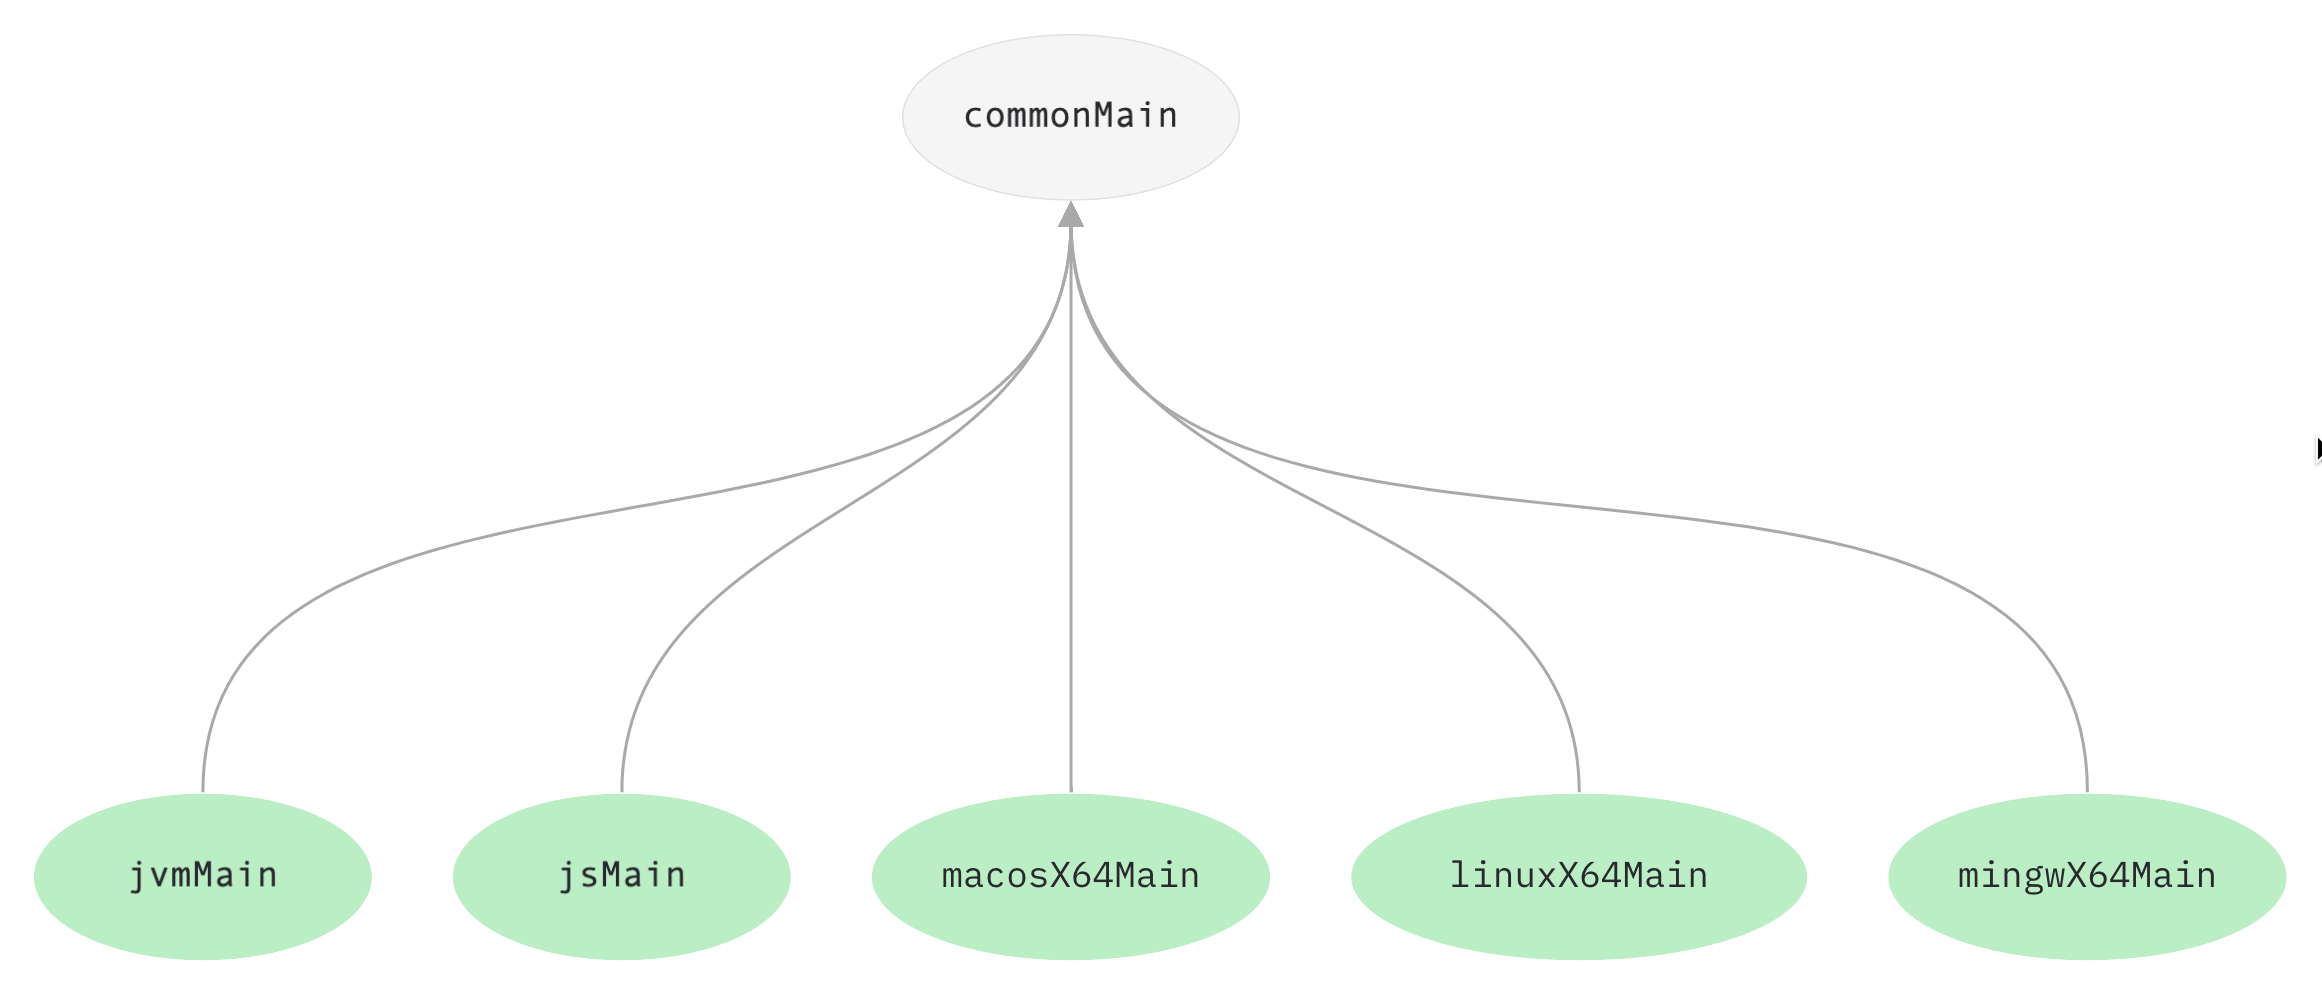
\includegraphics[width=\linewidth]{img/km-structure.png}
    \caption{Grafische voorstelling Kotlin Multiplatform en de verschillende platformen \autocite{Kotlin2021MP}}
    \label{fig:SVZkm-structure}
\end{figure}

Na de algemene uitleg rond KM en KMM kan er nu in meer detail gekeken worden naar KMM. Om deze uitleg te ondersteunen zal verwezen worden naar figuur \ref{fig:SVZkmm}. Deze figuur geeft een goed algemeen beeld van de structuur van KMM. De ‘shared code’ in de figuur verwijst hier naar Common Kotlin of CommonMain, dit is het gedeelde binnenin KM dat de gedeelde logica zal bevatten, dit was ook al zichtbaar op figuur \ref{fig:SVZkm-structure}. Daarnaast zal er nog per platform een aparte main zijn die de code zal implementeren. Hier in de figuur zal het project ook nog een iosMain en een kotlinMain, deze kunnen later ook nog uitgebreid worden met bijvoorbeeld een macosX64Main van KM. De situatie geïllustreerd in de figuur is een applicatie waar Kotlin Multiplatform Mobile gebruikt wordt. Deze zal zich speciaal richten op applicaties voor iOS en Android. Voor de communicatie tussen het common deel en de platform specifieke delen zal Kotlin gebruik maken van het expected/actual systeem. Hierbij worden binnenin de CommonMain elementen gedeclareerd met expect en de platform specifieke delen zullen dezelfde elementen declareren met actual. Deze structuur kan gebruikt worden voor functies, klassen, interfaces, enumeraties, properties en annotaties. 

\begin{figure}[h!]
    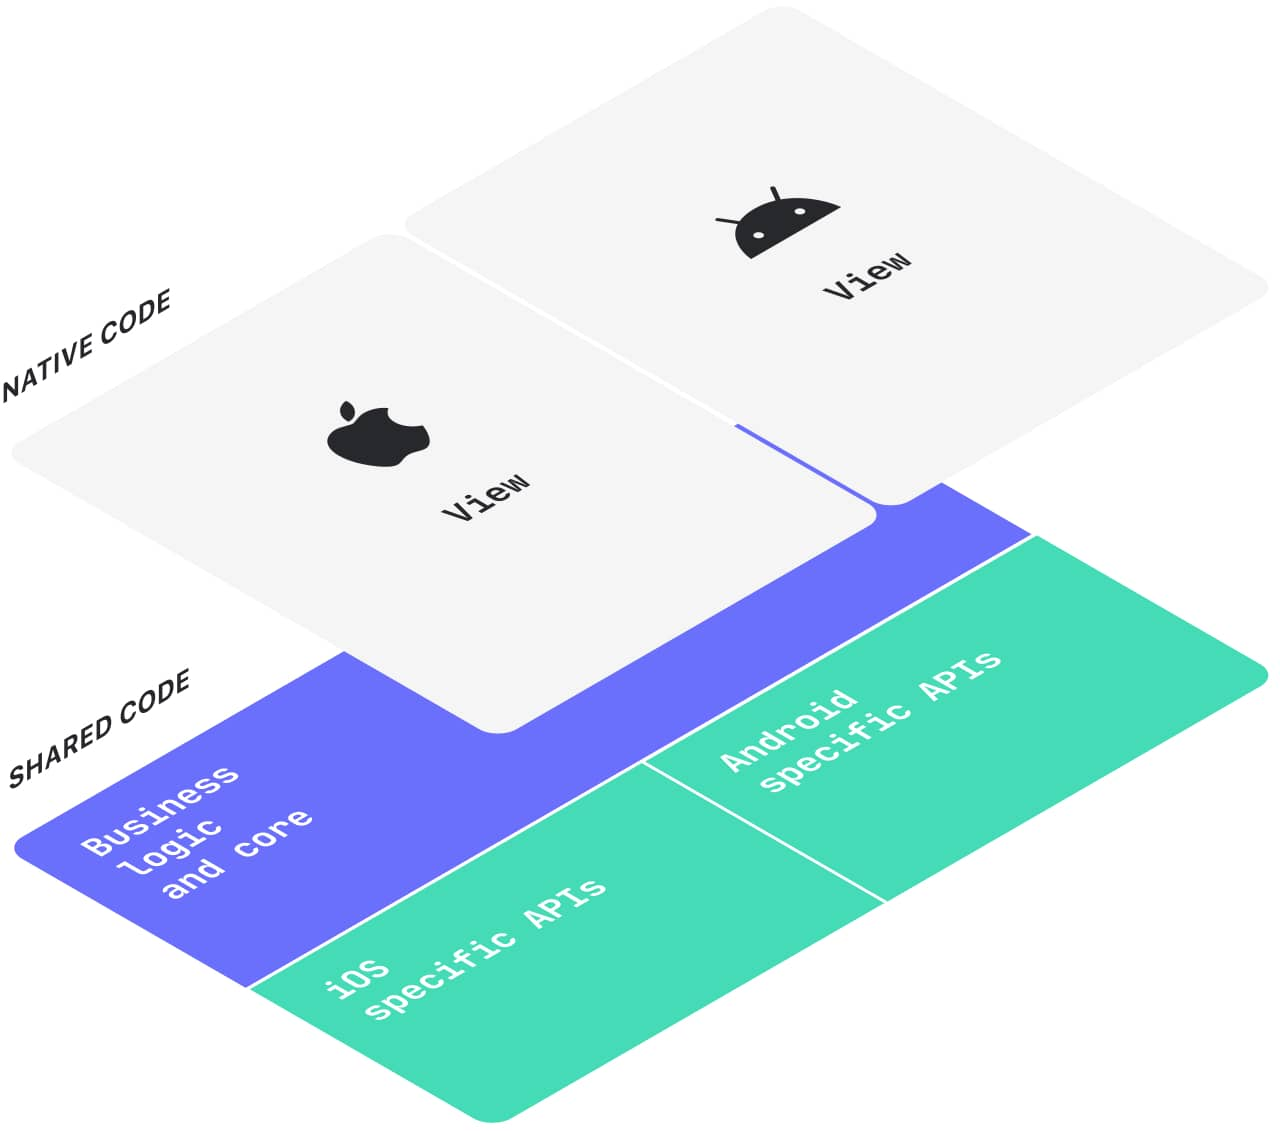
\includegraphics[width=\linewidth]{img/kmm.jpg}
    \caption{Grafische voorstelling Kotlin Multiplatform Mobile \autocite{KotlinKMM}}
    \label{fig:SVZkmm}
\end{figure}

In figuur \ref{fig:SVZkmm-code} kan bekeken worden hoe KMM geïmplementeerd zal worden binnen een project dat geschreven is voor de platformen iOS en Android. Bij de figuur kan ook volgende code teruggevonden worden in de documentatie van KMM.\autocite{Kotlin2021MP}

\begin{itemize}
    \item Code die in het common deel staat van KMM:
\begin{lstlisting}
    //Common
    expect fun randomUUID(): String
\end{lstlisting}
    \item Code die in het Android deel zal staan van de applicatie
\begin{lstlisting}
    //Android
    import java.util.*
    actual fun randomUUID() = UUID.randomUUID().toString()
\end{lstlisting}
     \item Code die in het iOS deel zal staan van de applicatie
 \begin{lstlisting}
     //iOS
     import platform.Foundation.NSUUID
     actual fun randomUUID(): String = NSUUID().UUIDString()
     
 \end{lstlisting}
\end{itemize}

\begin{figure}[h!]
    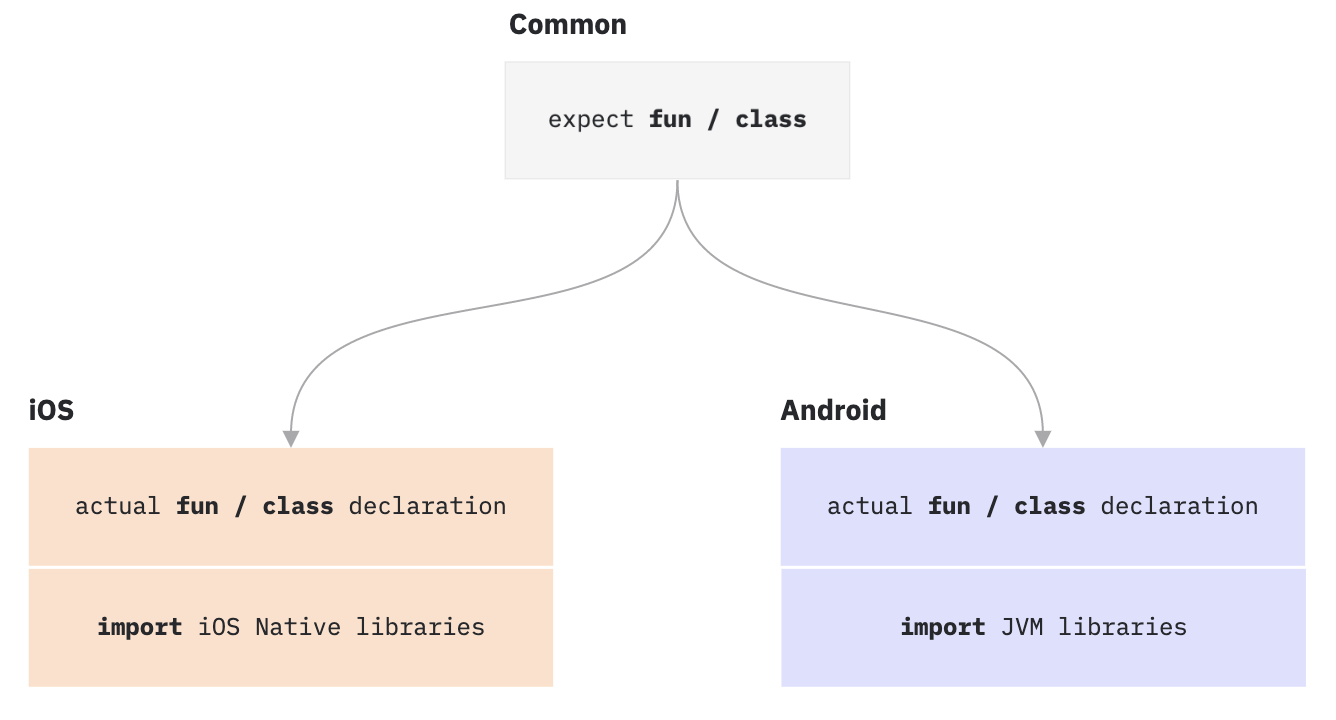
\includegraphics[width=\linewidth]{img/kmm-code.png}
    \caption{Grafische voorstelling van de code binnen KMM met iOS en Android als voorbeeld \autocite{Kotlin2021MP}}
    \label{fig:SVZkmm-code}
\end{figure}



\section{\IfLanguageName{dutch}{Kotlin Multiplatform versus alternatieven}{Kotlin Multiplatform versus alternatives}}
\label{sec:SVZKMMvsandere}

Nu duidelijk is wat Kotlin Multiplatform (KM) en Kotlin Multiplatform Mobile (KMM) omvat kan er bekeken welke andere alternatieven er zijn binnen het huidige landschap van cross-platform ontwikkeling. Een van de alternatieven die besproken zal worden is Flutter\footnote{flutter.dev}.

Flutter is een user interface toolkit ontwikkeld door Google en zit aan versie 1.22 sinds oktober 2020.\autocite{Sells2020} De toolkit richt zich op mobile, web en desktop applicaties en zal de code native compileren. Zoals reeds beschreven is Flutter een user interface toolkit en zal dus de user interface delen over de verschillende platformen. Hiervoor zal Flutter widgets gebruiken die geïnspireerd zijn door React.\autocite{FlutterWidgets} Dit impliceert dus dat hierbij de business logica zal moeten verwerkt worden per platform.

De ontwikkelaar van de cross-platform applicaties kan dus verschillende kanten uitgaan voor de ontwikkeling van de applicatie. Een eerste mogelijk is de reeds besproken technologie van KM en KMM hierbij zal de business logica gedeeld worden tussen de verschillende platformen. Het grootste voordeel aan deze manier van werken is dat de gebruiker een native ervaring zal hebben bij het gebruik van de applicatie. Daartegenover staat wel dat de user interface niet voor alle platformen hetzelfde is. Een andere mogelijke manier is het delen van de user interface, een besproken voorbeeld hiervan is Flutter. Deze manier zal als voordeel hebben dat alle applicaties op de verschillende platformen dezelfde look en feel zullen hebben, een nadeel is echter dat de business logica per platform verwerkt zal moeten worden.

\section{Testcriteria}
\label{sec:SVZtestcriteria}



Om een goede vergelijkende studie te maken is het belangrijk om op voorhand bepaalde testcriteria vast te leggen die gebruikt kunnen worden als maatstaf voor de geschreven applicaties. Hierbij is het belangrijk rekening te houden met het feit dat deze testcriteria van toepassing moeten zijn op zowel de native als cross-platform applicaties. Voor deze vergelijkende studie zijn volgende testcriteria gekozen en aan de hand van deze testcriteria zal gedocumenteerd worden hoe goed de cross-platform applicaties presteren ten opzichte van de native varianten. De testcriteria zijn: het aantal lijnen code, de compileersnelheid, de voetafdruk, de ontwikkeltijd,  de kostprijs. Deze testcriteria worden hieronder kort besproken. 

\begin{itemize}
    \item Aantal lijnen code
    \begin{itemize}
        \item Het totaal aantal lijnen code van een applicatie zal geëvalueerd worden over het gehele project. In het geval van native applicaties worden deze opgeteld bij elkaar.
    \end{itemize}
    \item Compileersnelheid
    \begin{itemize}
        \item Dit is de snelheid waarmee de specifieke applicatie zal kunnen compileren. Dit kan gemeten worden in de ontwikkelingssoftware voor de desbetreffende programmeertaal van de applicatie.
    \end{itemize}
    \item Voetafdruk
    \begin{itemize}
        \item Dit impliceert de omvang die de applicatie zal innemen op het platform waarvoor deze ontwikkeld is. Hiervoor kan de applicatie gebruikt worden die de ontwikkelingssoftware genereert.
    \end{itemize}
    \item Ontwikkeltijd
    \begin{itemize}
        \item Deze tijd beschrijft het aantal werkuren dat een ontwikkelaar nodig heeft om een specifieke applicatie te schrijven. Hierbij kan onder andere gebruik gemaakt worden van platformen zoals GitHub om deze tijd te meten of inschatten.
    \end{itemize}
    \item Kostprijs
    \begin{itemize}
        \item Hierbij wordt de geschatte kostprijs om een applicatie te laten ontwikkelen door een IT-bedrijf in kaart gebracht. Dit wordt berekend aan de hand van geschatte werkuren en een gemiddelde kostprijs per uur. Daarnaast wordt nagegaan of cross-platform een effect zal hebben op het systeem van vooraf bepaalde totaalprijzen indien bedrijven daarmee werken.
    \end{itemize}
\end{itemize}